% !TeX root = 06gy_cpp
\documentclass[../cpp_book/cpp_book.tex]{subfiles}
\begin{document}
	\onlyinsubfile{
		\begin{center}
			{\LARGE\textbf{C++}}
			
			{\Large Gyakorlat jegyzet}
			
			6. óra
		\end{center}
		A jegyzetet \textsc{Umann} Kristóf készítette \textsc{Horváth} Gábor gyakorlata alapján. (\today)
	}
	\subsection{Értékadó operátor}
  Az előző órán elkészült másoló konstruktor megoldotta a probléma egy részét, de az értékadással hasonló problémák merülnek fel. Hasonlóan a fordító által generált másoló konstruktorhoz, az alapértelmezetten az értékadás operátor (\textit{assignment operator}, vagy röviden \texttt{=}) is meghívja az egyes tagok értékadó operátorait, amik a primitív típusok esetén bitről bitre másolnak.
\begin{lstlisting}
struct List
{
	// ...
	
	// copy constructor
	List(const List &other) : data(other.data), next(0)
	{
		if (other.next != 0)
			next = new List(*other.next);
	}
	
	// assignment operator
	List& operator=(const List &other)
	{
		delete next;
		data = other.data;
		if (other.next) // if(other.next) == if(other.next != 0)
			next = new List(*other.next);
		else
			next = 0;
		return *this;
	}
	
	//...
};
\end{lstlisting}
	Az új értékadás operátor először kitörli az aktuális lista elemeit, majd rekurzív módon lemásolja az \texttt{other} elemeit.
	
  Kicsit részletesebben: az első lépés a \texttt{delete next;}, a fejelemet leszámítva felszabadítja az összes többi listaelemhez tartozó memóriaterületet, eztán lemásoljuk az \texttt{other} fejelemében lévő adatot. Végül a másoló konstruktorhoz hasonlóan rekurzív módon lemásoljuk az \texttt{other} farokrészét (amennyiben az létezik).
	
  Azáltal, hogy egy listaelem másolásakor az összes listaelem által birtokolt (heapen lévő) objektum is másolásra kerül, elértük azt, hogy a másolaton végzett módosításoknak ne legyen hatása az eredeti objektumra.
	\medskip
	
	Figyeljük meg, hogy az értékadás operátorban egy az adott objektumra mutató referenciával tértünk vissza. Ennek oka az, hogy szeretnénk, ha lehetséges lenne az értékadások láncolása:
	\begin{lstlisting}
			int a = b = c = d = 0; // a = (b = (c = (d = 0)))
	\end{lstlisting}
  Itt rendre (az operátorok kiértékelési sorrendjét tekintve) \texttt{d}-re, \texttt{c}-re, \texttt{b}-re, \texttt{a}-ra mutató referenciát ad vissza az értékadás operátor, így a végeredmény az lesz, hogy mindegyik változót 0-ra inicializáltuk.
	\begin{note}
    Miért nem konstans referenciával térünk vissza? Akkor nem csinálhatnánk hasonlót: (legyen \texttt{f(int \&)}) \texttt{f(a = 0)}.
	\end{note}
	
	Egyszerűsítsük a lista kiírását is!
	\begin{lstlisting}
struct List
{
	//...
	
	void print ()
	{
		std::cout << data << ' ';
		if (next)
			next->print();
	}
	
	//...
};
	\end{lstlisting}
	Ellenőrizzük, hogy az eredeti elemek nem változtak a másolás következtében!
	\begin{lstlisting}
int main ()
{
	List head(7);
	head.add(8);
	head.add(2);
	{
		List cHead = head;
	}
	head.print();
}
	\end{lstlisting}
	Kimenet: \texttt{7 8 2}
	
	Elértük, hogy biztonságos legyen a lista használata? Most már látszólag a másolás és az értékadás sem okozhat memóriakezeléssel kapcsolatos problémát. Van egy eset, amire a kód még nincs felkészítve! Mi történik, ha önmagának adjuk értékül a listát? Az első lépésben törlésre fog kerülni a fejelemet leszámítva minden elem. Eztán a következő lépésekben már felszabadított memóriaterületetről próbáljuk átmásolni a megfelelő adatokat. A \texttt{cHead = cHead} tehát use-after-free hibát fog okozni. Mennyire valós a félelem ettől a hibától? Hiszen nem gyakran adunk értékül egy objektumot önmagának! Tekintsük a következő függvényt:
	\begin{lstlisting}
void f(List &l1, List &l2)
{
	//...
	l1 = l2;
	//...
}
	\end{lstlisting}
	Ha valaki ugyanazt a listát adja meg mindkét paraméternek, akkor máris megvan a baj. Látható tehát, hogy ilyen jellegű hibát nem feltétlen olyan nehéz elkövetni.  Módosítsuk az értékadás operátorunkat oly módon, hogy ne okozzon problémát az önértékadás:
\begin{lstlisting}
List& operator=(const List &other)
{
	if (this == &other) return *this;
	delete next;
	if (other.next)
		next = new List(*other.next);
	else
		next = 0;
	return *this;
}
\end{lstlisting}
  Emlékezzünk, a \texttt{this} kulcssszó segítségével tudunk rámutatni tagfüggvényen belül az adott objektumra, amin a tagfüggvény meghívásra került. Tulajdonképpen arról van szó, hogy például a \texttt{head.print()} esetében enélkül a kulcsszó nélkül nem tudnánk \texttt{print()}-en belül \texttt{head}-re hivatkozni. Az objektum neve tagfüggvényen belül nem elérhető. A \texttt{this} egy pointerként is felfogható, mely a \texttt{head} objektumra mutat.
	\medskip

	Sikeresen létrehoztunk egy félig \textit{reguláris típust}.
	\medskip
	
	Egy \texttt{T} típus \textbf{reguláris típus}, ha van neki:
	\begin{enumerate}
		\item default konstruktora
		\item destruktora
		\item értékadás operátora, továbbá
		\begin{lstlisting}
T b;
T a;
a = b;
		\end{lstlisting}
		Ekkor \texttt{a} ekvivalens \texttt{b}-vel, és ha \texttt{a}-t módosítjuk, akkor \texttt{b} nem változik, és viszont.
		\item másoló konstruktora, továbbá
		\begin{lstlisting}
T b;
T a = b;
		\end{lstlisting}
		Ekkor \texttt{a} ekvivalens \texttt{b}-vel, és ha \texttt{a}-t módosítjuk, akkor \texttt{b} nem változik, és viszont.
		\item egyenlőségvizsgálat (\texttt{operator==}) (Ha nincs, akkor az adott típust félig regulárisnak nevezzük)
	\end{enumerate}
	\begin{note}
		Azt a másoló konstruktorral vagy értékadó operátorral történő műveletet, amikor a pointer adattagoknak úgy adunk értékül, hogy ne ugyanarra a területre mutassanak, \textit{deep copy}-nak hívjuk. Amikor ez nem történik meg, azt \textit{shallow copy}-nak nevezzük.
	\end{note}
	\subsection{Adattagok védettsége}
	Biztonságossá sikerült tenni a lista használatát? A felhasználó most már a megfelelő metódusok, valamint a másolás és értékadás használatával nem tud elkövetni memóriakezeléssel kapcsolatos hibát. Az adattagokhoz azonban továbbra is hozzá fér. Így, a következő módon továbbra is érhetik meglepetések:
	\begin{lstlisting}
int main()
{
	List head(8);
	head.add(7);
	head.add(2);
	head.next = 0;
}
	\end{lstlisting}
	Itt az első listaelem utáni elemeket lecsatoljuk, és azoknak a memóriája elszivárog. A probléma forrása az, hogy a \textbf{felhasználó hozzáfér az adattagokhoz.} A felhasználó így olyan állapotba állíthatja az adott objektumot, amire az objektum tagfüggvényei nincsenek felkészülve. Másik probléma, hogy a felhasználó azáltal, hogy hozzáfér az adattagokhoz, ki tudja használni a lista belső reprezentációját. Emiatt nehezebben fenntarthatóvá válik a kód, mivel a lista reprezentációját érintő változtatások esetén a felhasználói kódokat is módosítani kell. Példaképp, ha a \texttt{List} \texttt{next} adattagjának új nevet adunk, akkor át kéne írni minden olyan kódot ami \texttt{next}re hivatkozik.
	
	Jó lenne, ha hiába változna a belső reprezentáció, a kódnak nem kéne a felhasználói kódnak változnia. 
	
	Rejtsük el az adattagokat a felhasználó elől!

\begin{lstlisting}
class List // lehetne struct is
{
public:
	List(int data, List *next = 0) : //...
	void add(int data) {//...}
	List(const List &other) //...
	List& operator=(const List &other) {//...}
private:
	int data;
	List *next;
};
\end{lstlisting}
  Az osztály minden tagja, mely a \texttt{public} kulcsszó után jön, elérhető bárki számára. A \texttt{private} kulcsszó után következő adatok csak is kizárólag az adott osztályon belül érhető el (leszámítva a \texttt{friend}eket, de erről később).

	A \texttt{class} és a \texttt{struct} abban tér el, hogy alapértelmezetten a \texttt{struct} minden tagja publikus, míg \texttt{class}-nak privát. A \texttt{public} ill. \texttt{private} kulcsszóval mind a kettőnél explicit megadhatjuk a láthatóságot.
	\subsection{Iterátorok}
	Van egy súlyos következménye az imént bevezetett adatrejtésnek. Például, így nem tudunk hozzáférni a második elemhez kívülről. Vagy bármelyik másikhoz. Ilyenkor a naív megoldás az, ha módosítjuk a listát, és minden olyan függvényt, aminek hozzá kéne férnie az elemekhez, metódussá tesszük. Hiszen a lista metódusai hozzáférnek a privát adattagokhoz is.
	
	Ezt ugyanakkor nem akarjuk minden egyes függvénnyel megtenni. A végén nagyra nőne a lista osztály, ami nagyban rontja az kód érthetőségét és fenntarthatóságát. Emellett a reprezentáció változtatásával megint sok függvényt kellene módosítani.
	
	\medskip
	Próbáljunk találni egy megoldást erre a problémára. Figyeljük meg (feltéve hogy az adattagok még nem privátok) hogy így például végig tudnánk menni a lista elemein:
	\begin{lstlisting}
int main()
{
	List head(8);
	head.add(7); head.add(2);
	List *ptr = &head; //ptr első elemre mutat
	ptr = ptr->next; //második elemre
	ptr = ptr->next; //harmadik elemre
}
	\end{lstlisting}
	
	\begin{figure}[h]
		\centering
		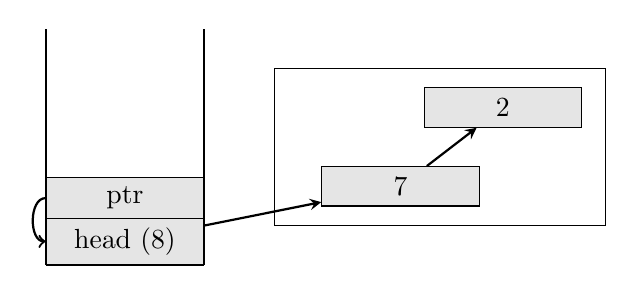
\begin{tikzpicture}
		\tikzstyle{Heap} = [rectangle, minimum width=4.2cm, minimum height=2cm, text centered, draw=black, fill=white]
		\tikzstyle{Stack} = [rectangle, minimum width=3cm, minimum height=1cm, text centered, draw=black, fill=white]
		\tikzstyle{ListNode} = [rectangle, minimum width=2cm, minimum height=5mm, text centered, draw=black, fill= gray!20]
		\tikzstyle{arrow} = [thick,->,>=stealth]
		
		\draw [thick, black] (-3, 0) -- (-1, 0);
		\draw [thick, black] (-3, 0) -- (-3, 3);
		\draw [thick, black] (-1, 0) -- (-1, 3);
		\node[Heap] at (2,1.5){};
		\node (7node) [ListNode] at (1.5,1) {7};
		\node (2node) [ListNode] at (2.8,2) {2};
		\node (ptr) [ListNode] at (-2,0.85) {ptr};
		\node (headNode) [ListNode] at (-2,0.3) {head (8)};
		
		\path[every node/.style={font=\sffamily\small}]
		(ptr) edge[bend right = 90, thick, ->] node [right] {} (headNode);
		\draw [arrow] (7node) -- (2node);
		\draw [arrow] (headNode) -- (7node);
		\end{tikzpicture}
		
		\bigskip
		\hspace{1.5mm} 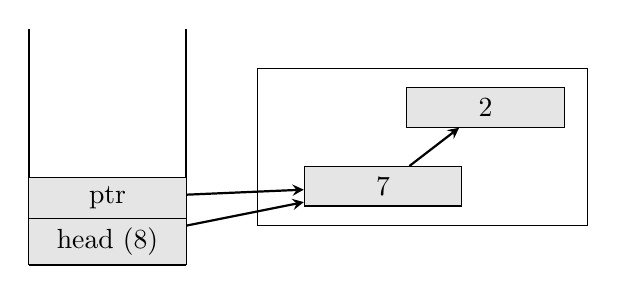
\begin{tikzpicture}
		\tikzstyle{Heap} = [rectangle, minimum width=4.2cm, minimum height=2cm, text centered, draw=black, fill=white]
		\tikzstyle{Stack} = [rectangle, minimum width=3cm, minimum height=1cm, text centered, draw=black, fill=white]
		\tikzstyle{ListNode} = [rectangle, minimum width=2cm, minimum height=5mm, text centered, draw=black, fill= gray!20]
		\tikzstyle{arrow} = [thick,->,>=stealth]
		
		\draw [thick, black] (-3, 0) -- (-1, 0);
		\draw [thick, black] (-3, 0) -- (-3, 3);
		\draw [thick, black] (-1, 0) -- (-1, 3);
		\node[Heap] at (2,1.5){};
		\node (7node) [ListNode] at (1.5,1) {7};
		\node (2node) [ListNode] at (2.8,2) {2};
		\node (ptr) [ListNode] at (-2,0.85) {ptr};
		\node (headNode) [ListNode] at (-2,0.3) {head (8)};
		\draw [arrow] (7node) -- (2node);
		\draw [arrow] (headNode) -- (7node);
		\draw [arrow] (ptr) -- (7node);
		\end{tikzpicture}
		
		\bigskip
		\hspace{4mm}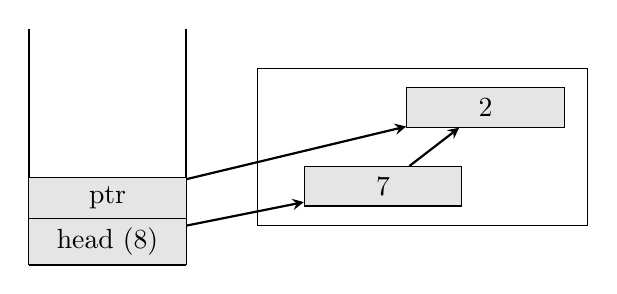
\begin{tikzpicture}
		\tikzstyle{Heap} = [rectangle, minimum width=4.2cm, minimum height=2cm, text centered, draw=black, fill=white]
		\tikzstyle{Stack} = [rectangle, minimum width=3cm, minimum height=1cm, text centered, draw=black, fill=white]
		\tikzstyle{ListNode} = [rectangle, minimum width=2cm, minimum height=5mm, text centered, draw=black, fill= gray!20]
		\tikzstyle{arrow} = [thick,->,>=stealth]
		
		\draw [thick, black] (-3, 0) -- (-1, 0);
		\draw [thick, black] (-3, 0) -- (-3, 3);
		\draw [thick, black] (-1, 0) -- (-1, 3);
		\node[Heap] at (2,1.5){};
		\node (7node) [ListNode] at (1.5,1) {7};
		\node (2node) [ListNode] at (2.8,2) {2};
		\node (ptr) [ListNode] at (-2,0.85) {ptr};
		\node (headNode) [ListNode] at (-2,0.3) {head (8)};
		\draw [arrow] (7node) -- (2node);
		\draw [arrow] (headNode) -- (7node);
		\draw [arrow] (ptr) -- (2node);
		\end{tikzpicture}
		\smallskip
		
		Pointer segítségével végig tudunk menni (iterálni) a lista elemein.
	\end{figure}
	A problémát tehát orvosolhatnánk azzal, hogyha ezt a pointert adattaggá tennénk, és metódusokon keresztül tudnánk léptetni, illetve az adott elemet lekérdezni. Ezt megoldhatjuk egy un. felsorolóval:
\begin{lstlisting}
class List
{
	//...
	
	void First() //pointert az első elemre állítja
	{
		cursor = this;
	}
	int& Current() //adott elem lekérdezése
	{
		return cursor->data;
	}
	void Next() //pointer léptetése a következő elemre
	{
		cursor = cursor->next;
	}	
	bool End() //a lista végére értük-e
	{
		return cursor == NULL;
	}
	
private:
	int data;
	List *next;
	List *cursor;
};
\end{lstlisting}
	Figyeljük meg, hogy \texttt{Current()} referenciával tér vissza, hogy ne \texttt{data} másolatát, hanem a \texttt{data}-ra hivatkozó referenciát kapjunk meg, így tudjuk a lista elemeinek az értékeit módosítani. Az \texttt{End} metódus azt vizsgálja meg, hogy a \texttt{cursor} nullpointer-e, lévén a lista utolsó eleme mindig nullpointer.
	\begin{note}
		Gyorsan megállapíthatjuk, hogy ha az \texttt{End} metóus igazat ad, akkor \texttt{Current} metódus egy nullpointer dereferálna, ami nem definiált viselkedés. Ez azonban nem probléma, hisz addigra a lista összes elemén végigiteráltunk. Tulajdonképpen azt is mondhatjuk, hogy ekkor \texttt{cursor} a lista ,,utolsó utáni elemére mutat''. 
	\end{note}
\begin{lstlisting}
for(head.Init(); !head.End(); head.Next())
	doSomething(head.Current());
\end{lstlisting}
	Első látásra a problémát orvosoltuk, tudunk a listákkal tárolt adatokkal dolgozni (pl. összeadni őket, stb). De egy rendezésnél már problémásabb. Ha csak egy kurzorunk van, nem tudunk egyszerre 2 elemhez hozzáférni, hogy összehasonlítsuk őket vagy megcseréljük őket. Egy lehetséges megoldás, ha még egy kurzort hozzáadunk a listához:
\begin{lstlisting}
class List
{
	//...
	
	void First()
	{
		cursor = this;
	}
	int& Current()
	{
		return cursor->data;
	}
	void Next()
	{
		cursor = cursor->next;
	}	
	bool End()
	{
		return cursor == 0;
	}
	
	void First2()
	{
		cursor2 = this;
	}
	int& Current2()
	{
		return cursor2->data;
	}
	void Next2()
	{
		cursor2 = cursor2->next;
	}	
	bool End2()
	{
		return cursor2 == 0;
	}
	
private:
	int data;
	List *next;
	List *cursor;
	List *cursor2;
};
\end{lstlisting}
	Ezzel már egy rendezést meg tudunk oldani. De talán érezhető, hogy ez nem a legszebb megoldás. Ha három \texttt{cursor} kéne egy algoritmushoz, akkor megint bajban lennénk. Ennél létezik sokkal szofisztikáltabb megoldás: az \textbf{iterátorok}.
	
	Az iterátorok a pointerek általánosításai, segítségükel tudunk végigiterálni egy konténer elemein (azaz velük tudjuk lekérdezni a konténer elemeit). A problémát orvosolandó, külön osztályt is fognak kapni.
	
	Amíg amíg a kurzor adattag volt, könnyedén meg tudtuk adni a konténerünk első és utolsó elemét, azonban ezt most máshogy kell megoldanunk. Először is, állapodjunk meg abban, hogy leendő iterátorunk neve \texttt{Iterator} legyen. Mivel tudjuk, hogy lényegében egy pointert fogunk osztályba csomagolni, már valami ötletünk lehet arról, hogyan fog kinézni:
	\begin{lstlisting}
class List {/* ... */};

class Iterator
{
public:
	Iterator(List *_p) : p(_p) {}
	bool operator==(Iterator &other)
	{
		return p == other.p;
	}
	bool operator!=(Iterator &other)
	{
		return !(*this == other);
	}
	//TODO: kéne valami a léptetésre, adott elem lekérdezésére
private:
	List *p;
};

	\end{lstlisting}
	\begin{note}
		Figyeljük meg, hogy a \texttt{!=} operátor meghívja a \texttt{==} operátort, és negálja. Ha bármikor módosulna az iterátorunk implementációja, elég lesz \texttt{==} operátort módosítani.
	\end{note}
	A megoldás az lesz, hogy nem az \texttt{Iterator}, hanem a \texttt{List} osztályban fog szerepelni a lista elejét és hátulját lekérdező metódus:
	\begin{lstlisting}
class List
{
	//...
public:
	Iterator begin()
	{
		return Iterator(this);
	}
	Iterator end()
	{
		return Iterator(0);
	}
};

class Iterator {/* ... */};
	\end{lstlisting}
	 A \texttt{head.begin()} vissza fog adni egy iterátort, ami a \texttt{head} a legelső elemére mutat, \texttt{head.end()} az utolsó utáni elem. Az iterátor osztályból már csak a lépegetés és az adott elem lekérdezése hiányzik, melyeket a \texttt{++} és a \texttt{*} operátorok túlterhelésével fogunk megoldani. Megállapítható, hogy \texttt{Iterator} kielégíti az un. \textbf{forward iterátor} követelményeit:

	Egy \texttt{T} típus \textbf{forward iterator}, ha rendelkezik:
	\begin{enumerate}
		\item \texttt{++} operátorral
		\item egyenlőség vizsgáló operátorral \texttt{==}
		\item egyenlőtlenség vizsgáló operátorral \texttt{!=}
		\item dereferáló operátorral \texttt{*}
	\end{enumerate}
	Sajnos azonban fordítási hibát kapunk. Hova írjuk az \texttt{Iterator} osztályt? Hiszen ha a lista elé tesszük, az \texttt{Iterator} nem fogja tudni, hogy mi az a \texttt{List}. Ha utána tesszük, nem fogja tudni a \texttt{List} hogy mi az az \texttt{Iterator}. Erre szükség van a listában az \texttt{end} és a \texttt{begin} metódus megírásához. A körkörös függőség feloldása érdekében \textbf{forward deklarálni} fogunk. 
	\begin{lstlisting}
class List; //forward declaration

class Iterator {/* ... */};

class List {/* ... */};
	\end{lstlisting}
	A fordító ezek után nem fog arra panaszkodni, hogy a \texttt{List} egy ismeretlen azonosító (\textit{incomplete type}). A forward deklaráció azt mondja a fordítónak, hogy a \texttt{List} később, akár egy másik fordítási egységben definiálva lesz. Amíg egy pointerrel csak az adott memóriaterületre mutatunk, de rajta keresztül nem akarunk műveletek végrehajtani (azaz, nem akarjuk a pointert dereferálni) addig nem szükséges az adott osztályt definiálni. (Például így lehet az, hogy minden pointer mérete egyenlő.)
	
	\medskip
	Még hiányzik a \texttt{++} és a \texttt{*} operátor. Ez előbbi esetében ne felejtsük el, hogy egy pointer léptetése esetén visszakapjuk az adott obejktumot (azaz, \texttt{*++ptr = 5} helyes, hisz \texttt{++ptr} visszaadja \texttt{ptr}-t), így a mi operátorunkkal is így kéne eljárni.
\begin{lstlisting}
class List;

class Iterator
{
public:
	Iterator(List *_p) : p(_p) {}
	bool operator==(Iterator &other)
	{
		return p == other.p;
	}
	bool operator!=(Iterator &other)
	{
		return !(*this == other);
	}
	Iterator operator++()
	{
		p = p->next;
		return *this;
	}
	int& operator*()
	{
		return p->data;
	}
private:
	List *p;
};

class List {//...};
\end{lstlisting}
	Amennyiben az előbb említett operátorokat az \texttt{Iterátor}on belül fejtjük ki, pont az előbb említett hibát követjük el: dereferáltuk \texttt{p}-t, melyhez ismerni kéne az osztály implementációját. A forward deklaráció miatt a fordító tudja már, hogy a \texttt{List} az egy osztály, de nem tudja ellenőrizni, hogy \texttt{next} adattaggal rendelkezik-e. Ezért ezeknek a tagfüggvényeknek szét kell választani a deklarációját és definícióját úgy, hogy a definíció a \texttt{List} kifejtése után szerepeljen:
\begin{lstlisting}
class List;

class Iterator
{
public:
	Iterator(List *_p) : p(_p) {}
	bool operator==(Iterator &other)
	{
		return p == other.p;
	}
	bool operator!=(Iterator &other)
	{
		return !(*this == other);
	}
	Iterator operator++();
	int& operator*();
private:
	List *p;
};

class List {//...};

//hivatkoznunk kell arra, hogy operator++ Iterator egy metódusa
Iterator Iterator::operator++()
{
	p = p->next;
	return *this;
}
int& Iterator::operator*()
{
	return p->data;
}
\end{lstlisting}
  Felmerül még egy probléma: a \texttt{next} és \texttt{data} private adattagok. Az \texttt{Iterator} nem fér hozzá! Erre megoldás, ha \textbf{barát} (\textit{friend}) osztálya lesz az Iterátor a \texttt{List}nek.
	\begin{lstlisting}
class List
{
	//...
	friend class Iterator;
	//...
}
	\end{lstlisting}
	A barátként deklarált osztályok és függvények hozzá tudnak férni az osztály privát adattagjaihoz is.
	
	\smallskip
	Ezzel készen is van az iterátorunk, azonban ne feledjük el, hogy az \texttt{Iterator} csak egy pointer osztályba csomagolva, mellyel hozzá tudunk férni a lista elemeihez. Az előbb említett probléma, miszerint minden függvény ami a listához hozzá akar férni tagfüggvénnyé kéne tenni, megoldódott: példaképp a \texttt{print()}-et tagfüggvényből szabad, osztályon kívüli függvényt csinálhatunk.
 	
 	Amennyiben lehetőségünk van egy függvényt szabad (osztályon kívüli) függvényként megírni, érdemes élni a lehetőséggel. Ezáltal az osztályaink kisebbek és könnyebben érthetőek lesznek.
	\begin{lstlisting}
void print(List &l)
{
	for(Iterator it = l.begin(); it != l.end(); ++it)
	{
		std::cout << *it << ' ';
	}
	std::cout << std::endl;
}
	\end{lstlisting}
	Ez a függvény, csak úgy mint az \textit{STL} függvények is, balról zárt, jobbról nyitott $[\ )$ intervallummal dolgozik. Azaz az \texttt{end()} már nem eleme a listának, az az utolsó {utáni} elem (\textit{past-the-end iterator}).
	
	\medskip
	Nézzük meg, hogy miért jobb az iterátor, mint a felsoroló. Annyi \texttt{Iterator}-t hozunk létre, amennyit csak akarunk, nem vagyunk korlátozva a \texttt{cursor}ok darabszáma által. Az iterátorok emellett tetszőlegesen tárolhatóak, átadhatóak függvényeknek. Nincs elrejtve az objektum belsejébe. Továbbá, tudjuk módosítani a listában található elemeket anélkül, hogy a lista reprezentációját ismernünk kellene. Egy iterátorokat használó kód módosítása nélkül megváltoztatható a lista belső reprezentációja. Ez lehetővé teszi azt, hogy több programozó csapatban dolgozzon, egymástól független kódrészleteket úgy tudjon módosítani, hogy ne kelljen egymás kódját átírni.
	
	\medskip
	Azon metódusok, amik után \texttt{const} kulcsszó szerepel nem tudják megváltoztatni az adott osztály adattagjait. Ezeket a metódusokat \textbf{konstans metódusok}nak (\textit{const method}) hívják. Egy konstans objektumon csak akkor lehet meghívni egy metódust, ha az a metódus konstans.
	
	\medskip
	Megfigyelhető, hogy \texttt{print} nem módosítja a paraméterként kapott listát, így átvehetnénk konstans referenciával is. Ennek az eredménye fordítási hiba: az \texttt{end} és \texttt{begin} nem konstans metódusok, hiszen ami iterátort visszaad, azokon keresztül tudjuk módosítani az objektumot.
	\begin{note}
		Ami lehet \texttt{const}, az \textbf{legyen} \texttt{const}! Például, rögtön megállapítható hogy az \texttt{Iterator} osztály \texttt{==} és \texttt{!=} operátorai nyugodtan lehetnek konstans metódusok is.
	\end{note}
	\subsection{Konstans iterátorok}
	Erre a megoldás, ha konstans iterátort is írunk, ami egy konstans\textbf{ra} mutató pointer általánosítása.
\begin{lstlisting}
class List;

class Iterator {/* ... */};

class ConstIterator
{
public:
	Const Iterator(const List *_p) : p(_p) {}
	bool operator==(ConstIterator &other) const
	{
		return p == other.p;
	}
	bool operator!=(ConstIterator &other) const
	{
		return !(*this == other);
	}
	ConstIterator operator++();
	int operator*() const; //nem referenciával tér vissza!
private:
	const List *p; //konstanra mutató pointer!
};

class List
{
	//...
	ConstIterator begin() const
	{
		return ConstIterator(this);	
	}
	ConstIterator end() const
	{
		return ConstIterator(0);	
	}
	
	friend class ConstIterator;
	//...
};

Iterator Iterator::operator++() {/* ... */}
int& Iterator::operator*() {/* ... */}

ConstIterator ConstIterator::operator++()
{
	p = p->next;
	return *this;
}
int ConstIterator::operator*() const
{
	return p->data;
}
\end{lstlisting}
	\begin{note}
		Ahogy az korábban említve volt, azok a tagfüggvények, melyek konstansságban nem egyeznek meg (pl. az \texttt{Iterator}-ral visszatérő \texttt{begin} és \texttt{end} tagfüggvények nem konstansok, míg a \texttt{ConstIterator}-ral visszatérő \texttt{begin} és \texttt{end} azok), azok különböző függvények számítanak (azaz, a \texttt{begin} és az \texttt{end} két-két overload-dal rendelkeznek).
	\end{note}
	Egy \texttt{const List} típusú objektumon csak a konstans metódusok hívhatóak meg, így a meghívott \texttt{begin()} visszatérési értékének típusa \texttt{ConstIterator} lesz. Egy nem konstans \texttt{List} objektumnál viszont \texttt{Iterator} lesz.
	\begin{lstlisting}
int main()
{
	List head(8); //nem const
	head.add(7);
	head.add(2);
	{
		ConstIterator cit = head.begin(); //hiba
	}
}
	\end{lstlisting}
	Két különböző típust nem tudunk egymásnak értékül adni, ha nem létezik köztük konverzió. Mivel nem konstansra mutató mutató konvertálódhat konstansra mutató mutatóvá, ezért természetes lenne hasonló konverziót az iterátorok közt is bevezetni. Ezt egy új konstruktor segítségével tehetjük meg:
	\begin{lstlisting}
class ConstIterator
{
	//...
public:
	ConstIterator(Iterator &other) : p(other.p) {}
	//...
};
	\end{lstlisting}
	Emlékezzünk, hogy az \texttt{Iterator}-nak a \texttt{p} adattagja privát. A forduló kódhoz egy friend deklaráció bevezetése szükséges!
	
	Meglepő lehet, hogy az értékadás egy új konstruktor bevezetését követően le fog fordulni. A \texttt{head.begin()} a fenti esetben egy \texttt{Iterator}-t ad vissza, mivel \texttt{head} nem konstans! Eztán a fordító az imént megírt konstruktor segítségével az \texttt{Iterator} típusú változóból készít egy \texttt{ConstIterator} típusút. Ezzel \textit{implicit kódon átkonvertálja} \texttt{Iterator}-t \texttt{ConstIterator}-rá, és utána hívja meg a másoló konstruktort. 
	
	\subsection{Explicit konstruktorok}
	Azt, hogy az egy paraméteres konstruktorokat a fordító implicit konverzióra felhasználja a fenti módon, megtilthatjuk itt is, ha \texttt{explicit} kulcsszót írunk a konstruktor elé.
	
	\begin{lstlisting}
class ConstIterator
{
	//...
public:
	explicit ConstIterator(Iterator &other) : p(other.p) {}
	//...
};
	\end{lstlisting}
	Jelen esetben nem akarjuk a konverziót megtiltani, lévén az \texttt{Iterator} és a \texttt{ConstIterator} hasonló feladatot lát el. Nézzük meg az eddigi kódjainket. Okozhat valahol meglepetést egy konverzió? A \texttt{List} egyik konstruktra gyanús lehet. Ha egy függvény listát vár paraméterül, egy darab \texttt{int}-et is elfogad, hisz a \texttt{List} konstruktorát felhasználva tudott volna csinálni abból az \texttt{int}-ből egy egy elemű listát! Ezt elkerülendő, tegyük a \texttt{List} konstruktorát \texttt{explicit}-té.
	\begin{lstlisting}
class List
{
public:
	explicit List(const int _data, List *_next = 0) : data(_data), next(_next) {}
	//...
};
	\end{lstlisting}
	\subsection{Konverziós operátor}
	Más módon is át lehet konvertálni egy \texttt{Iterator} típusú objektumot \texttt{ConstIterator} típusúvá. Azzal, hogy létrehozunk egy un. \textbf{konverziós operátor}t (\textit{conversion operator} vagy \textit{user defined conversion}). 
	\begin{lstlisting}
// ...
class ConstIterator; //forward deklaráció itt szükséges

class Iterator
{
public:
	// ...
	operator ConstIterator() const; //konverziós operátor
	// ...
};

class ConstIterator{//...}

Iterator::operator ConstIterator() const
{
	return ConstIterator(p);
}
// ...
	\end{lstlisting}
	A fenti konverziós operátor segítségével implicit módon végre lehet hajtani a konverziót. 
	\begin{lstlisting}
ConstIterator cit2 = head.begin(); //ok
	\end{lstlisting}	
	Amennyiben azt szeretnénk, hogy a konverzió létezzen, de implicit módon ne jöjjön létre, használhatjuk az \texttt{explicit} kulcsszót. Ez a kulcsszó azonban csak C++11 óta használható ilyen módon:
	\begin{lstlisting}
class Iterator
{
public:
	// ...
	explicit operator ConstIterator() const;
	// ...
};
	\end{lstlisting}
	Nézzünk meg pár példát, hogyan lehet a konverziót explicit módon használni:
	\begin{lstlisting}
int main()
{
	List head(8);
	ConstIterator cit1 = head.begin(); // hiba
	ConstIterator cit2 = ConstIterator(head.begin()); // ok
	ConstIterator cit3 = static_cast<ConstIterator>(head.begin()); // ok
}
	\end{lstlisting}
	\begin{note}
		A fent látható \texttt{static\_cast}-ról később lesz részletesen szó.
	\end{note}
	\begin{note}
		A fenti módosítások ismét csak gyakorlás célját képezték, az elkészítedő listának nem lesz része a konverziós operátor.
	\end{note}
	\begin{note}
    Amikor lehetőségünk van rá, használjunk egy paraméteres konstruktorokat a konverzióra. Amennyiben ahhoz az osztályhoz, amivé konvertálni szeretnénk, nem adhatunk hozzá új konstruktort (például könyvtári osztály), akkor használjuk a konverziós operátort. 
	\end{note}
\end{document}
